% TODO: Re-enable twopage when printing
\documentclass[12pt,a4paper]{report}

\usepackage{graphicx,color}
\usepackage{subfigure}
\usepackage{amsmath}
\usepackage{amsfonts}
\usepackage{amssymb}
\usepackage{listings}
\usepackage{xspace}
\usepackage{paralist}
\usepackage{array}
\usepackage{booktabs}
\usepackage{mdframed}

% Allows multiple titles.
\usepackage{titling}

% For displaying directory trees.
\usepackage{dirtree}

% Needed to rename {algorithm} wrapped {algorithmic} sections.
\usepackage{float}

% Used for theorem formatting.
\usepackage{amsthm}

% Graphs & figures.
\usepackage{tikz}
\usetikzlibrary{arrows,backgrounds,snakes}

% Line spacing
\usepackage{setspace}

\usepackage[numbers, sort&compress]{natbib}

% hyperref redefines a number of macros, so it should be last.  Empirically,
% doing so eliminates compiler warnings.
\usepackage[bookmarks, colorlinks]{hyperref}
% According to the hyperref readme, algorithm must follow hyperref

\usepackage{algorithm}
\usepackage[noend]{algpseudocode}
\usepackage{varwidth}

%~~~~~~~~~~~~~~~~~~~~~~~~~~~~~~~~~~~~~~~~~~~~~~~~~~~~~~~~~~~~~~~~~~~~~~~~~~~~~~
% Macros

% English
\newcommand{\cf}{\hbox{\emph{cf.}}\xspace}
\newcommand{\deletia}{\ldots [deletia] \ldots}
\newcommand{\etal}{\hbox{\emph{et al.}}\xspace}
\newcommand{\eg}{\hbox{\emph{e.g.}}\xspace}
\newcommand{\ie}{\hbox{\emph{i.e.}}\xspace}
\newcommand{\scil}{\hbox{\emph{sc.}}\xspace} %scilicet: it is permitted to know
\newcommand{\st}{\hbox{\emph{s.t.}}\xspace}
\newcommand{\wrt}{\hbox{\emph{w.r.t.}}\xspace}
\newcommand{\etc}{\hbox{\emph{etc.}}\xspace}
\newcommand{\viz}{\hbox{\emph{viz.}}\xspace} %videlicet: it is permitted to see
\newcommand{\vs}{\hbox{\emph{vs.}}\xspace}

\newcommand{\todo}[1]{{\color{red}(TODO: #1)}}

\newcommand{\ourtitle}{Smashing Heisentests}

\newcommand{\splatter}{Splatter}
\newcommand{\flaky}{flaky}


\newcommand\bench[1]{\textsf{\small #1}}

% Maths operators
\DeclareMathOperator*{\eq}{=}

%% Document-specific hyperref options
\hypersetup{
pdftitle={\ourtitle},
    pdfauthor={Earl T. Barr and Morrison Cole},
    plainpages=false,
    linkcolor=blue, % Overriding these colors to black is somewhat unfortunate
    %citecolor=black, % b/c the defaults are useful in color.
    citecolor=blue, % b/c the defaults are useful in color.
    filecolor=black,
    urlcolor=blue
}
\def\sectionautorefname{Section}
\def\subsectionautorefname{Section}
\def\subsubsectionautorefname{Section}
\newcommand{\subfigureautorefname}{\figureautorefname} %for subfigures
\newcommand{\defref}[1]{\hyperref[#1]{Definition~\ref*{#1}}}
\renewcommand{\algref}[1]{\hyperref[#1]{Algorithm~\ref*{#1}}}
\newcommand{\lineref}[1]{\hyperref[#1]{Line~\ref*{#1}}}

% Paragraph formatting
\setlength{\parskip}{\baselineskip}
\setlength{\parindent}{0pt}

% Line spacing
\onehalfspacing

%% lstlisting
\lstset{
	basicstyle=\ttfamily\small,
	numbers=left,
	language=Java,
	captionpos=b,
	breaklines=true,
	escapeinside={(*@}{@*)},
	breakatwhitespace=true
}

\pagestyle{plain}
\pagenumbering{arabic}

\begin{document}

\label{sec:title}

\begin{titlepage}
\begin{center}

{\huge \bfseries Smashing Heisentests \\[3cm]}

\textsc{\LARGE Morrison Cole}\\[0.5cm]
\textsc{\large BSc Computer Science}\\[0.3cm]
\textsc{\large Submission date: \today}\\[2cm]

\textsc{\LARGE Supervisor: Earl Barr}\\[0.5cm]
\textsc{\LARGE External Supervisor: Colin Vipurs}

\vfill

{\itshape This report is submitted as part requirement for the BSc Degree in Computer Science at UCL. It is substantially the result of my own work except where explicitly indicated in the text.}

{\itshape The report will be distributed to the internal and external examiners, but thereafter may not be copied or distributed except with permission from the author.}

\end{center}
\end{titlepage}


\begin{abstract}

We present a framework for identifying and accelerating the resolution of flaky test cases in a test suite. A flaky test case is one whose outcome is sensitive to some unknown input.

The framework operates on a continuous lifecycle. To begin, each test's probability of failure is calculated. Then, each test is adaptively instrumented with respect to a budget --- state-logging probes are placed in choice locations. Finally, aggregated data is analysed to identify predicates strongly associated with test failure. At each stage, the framework can work autonomously or with input from a developer.

Our instrumentation approach applies bug isolation techniques in an ideal environment, allowing us to record and analyse a huge amount of runtime data over time. We improve probe placement by taking into account control flow graphs and loops. Finally, we introduce the notion of an instrumentation budget and allocate probes based on learned cost.

We discuss and document the implementation of a working proof of concept, named \textit{\splatter}, that targets Android applications and integrates with a popular open-source continuous integration tool. We present preliminary results from the use of the tool on tests from a commercial product's test suite.

\end{abstract}


%% Contents. Perhaps use figures / tables.

% Force top-level sections to enumerate with natural numbers even on the 'report' type document.
\renewcommand\thesection{\arabic{section}}

\tableofcontents
\newpage
%\listoffigures
%\listoftables

% Makes all pages the height of the text on the page. No extra vertical space is added.
\raggedbottom

\noindent``\textit{Left uncontrolled, non-deterministic tests can completely destroy the value of an automated regression suite.}''

\hfill Martin Fowler

\section{Introduction}
\label{sec:intro}

\textit{The following are placeholders; subsections are to be removed.}

\subsection{Testing is used in practice across the industry}

Testing is as much a part of modern software development as deployment. Enforces quality, prevents regressions, reduces need for manual testing in certain areas.

\subsection{Testing is flawed/not always reliable}

Flaky tests across the industry.

\subsection{What we intend to do}

Apply adaptive bug isolation techniques to testing to gather information on flaky test cases with the aim of aiding their stabilization.

\subsection{How the rest of the paper is structured}
\section{Context}
\label{sec:context}

This section presents definitions and background information necessary for a
full understanding of the problem.


\subsection{\Flaky Tests}
\label{sec:sec:flaky_tests}

A test consists of a set of inputs and a corresponding expected output, over
some subject under test. In a perfect world, a test always produces the expected
output provided the subject's behaviour is fixed. In reality, environmental and
chance factors can affect the actual output. We can model the expected output
probabilistically.

\begin{quote}
	A \flaky test is one known to fail with low probability.
\end{quote}

\begin{defn}[\Flaky Test]
\label{def:flaky_test}

Let $\vec{I}$ be the lifting of all inputs, including coin flips and
environmental interactions, into a single input vector. $\vec{O}$ is the
corresponding desired output. Given a subject under test $f: \vec{I} \rightarrow
\vec{O}$, a test case is $(\vec{i},\vec{o})$. A \emph{\flaky test case} is one
where
%
\begin{align*}
  p(f(\vec{i}) \ne \vec{o}) = \epsilon
\end{align*}
%
for non-negligible probability $\epsilon \in (0..\alpha]$.

\end{defn}

Flaky tests fail rarely.  What is {\lq}rare{\rq} depends on the problem and the
cost of the test.  If a test fails frequently enough, it can be converted into a
standard failing test by repeatedly running the test, subject to the cost of
that test.  The parameter $\alpha$ represents this threshold between
reproducible via repetition and not.  The exact probability $\epsilon$ must be
non-negligible so that repeated trials are likely to trigger the failure.  In
practice, this constraint is easily met, since it is hard to imagine that a
negligible $\epsilon$ matters.  Combined with our budget $B$, we can determine
what values of $\epsilon$ we can afford to detect.

Figure~\ref{fig:flakiness} depicts \flaky tests in terms of probability of
failure.

\begin{figure}[h]
\begin{center}
	% See: http://www.texample.net/tikz/examples/line-plot-example/
	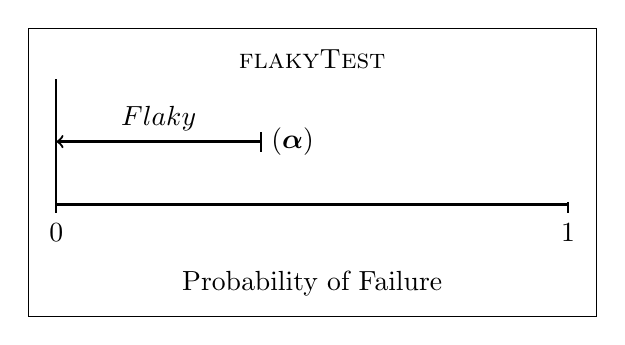
\begin{tikzpicture}[thick, framed, x=6.5cm, y=1.6cm]
		% Title
		\draw (0.5, 1) node[above] {$\textsc{\flaky Test}$};

		% Axis
		\draw (0,0) -- coordinate (x axis mid) (1,0);
	    \draw (0,0) -- coordinate (y axis mid) (0,1);

	    % Axis Labels
	    \node (padding) [below] at (0.4, 0) {};
		\node[below of = padding] at (x axis mid) {Probability of Failure};

	    % Ticks
	    \foreach \x in {0, 1}
	    	\draw (\x, 1pt) -- (\x, -3pt) node[anchor=north] {\x};

		% \flaky test range
	    \draw[<-] (0, 0.5) -- (0.4, 0.5); % Draw horizontal line
	    \draw (0.4, 0.42) -- (0.4, 0.58); % Draw right vertical tab

	    % Flakiness label
	    \node [above] at (0.2, 0.5) {$Flaky$};

	    % Alpha label
	    \node [right] at (0.4, 0.5) {$(\boldsymbol{\alpha})$};
	\end{tikzpicture}
\end{center}
\caption{}
\label{fig:flakiness}
\end{figure}


\subsection{Automated Testing}
\label{sec:sec:automated_testing}

Automated testing has been adopted by developers globally, from those working in
start ups to those in major corporations. As the number of environments
deployments are expected to run in increases, testing all possible variants
quickly becomes unworkable. It is impractical to manually test an application
across hundreds of devices every time it is modified. Automated tests serve a
simple purpose --- ensure the software under test behaves as expected in the
supported set of environments. A good test suite achieves this by exercising
discrete chunks of the program's code to ensure it behaves in some expected way.
At a high level, each test can be broken into three steps - arrangement, action
and assertion.

Anecdotally, the higher-level the behaviour being tested, the more likely a test
is to fail due to inputs unaccounted for. Tests that exercise seemingly valid
code can fail unexpectedly and unpredictably. Developers working with such tests
face a dilemma --- {\lq}suppress{\rq} the tests until they are fixed, or
acknowledge them but keep them active, potentially randomly breaking the build
from time to time until they are fixed. Since the tests exercise behaviour which
is needed (and indeed, works as intended), both solutions are workarounds until
the tests can be resolved. A set of tests displaying seemingly random failure
can devalue an entire suite, so it is of utmost importance that developers fix
such issues as they arise. The test suite is not a user-facing feature and can
quickly become a cost rather than a benefit.

In our experience, within the context of real software development projects
developers quickly become frustrated when dealing with \flaky tests and begin to
rely on instinct in order to stay productive. In other words, they lose
confidence in the test suite. It is essential to maintain a reliable test suite
for it to remain a beneficial part of a team's workflow.


\subsection{Why Not {\lq}Non-Deterministic{\rq}?}

Nondeterministic has three possible meanings depending on the context. In
existing literature, practitioners tend to use non-deterministic in the Physics
sense --- \ie, probabalistic. Given that nondeterministic has different meanings
in Computer Science and Statistics/Probability, it is better to avoid confusion
and choose a suitable term: \flaky.


\subsection{Fixing \Flaky Tests the Manual Way}

Sometimes, it is not possible to fix a \flaky test from the information output
by the testrunner alone. Typically, the information includes logs, an assertion
failure message and/or a stack trace. Applications with a user interface may
also provide a number of screenshots. Often, a developer will have to manually
gather information to build up an understanding of the intended flow versus the
actual flow on failing runs. For \flaky tests with a low failure rate, this can
be a painstaking and time-consuming process, if not completely ineffective.
Indeed, if the \flaky test is a timing based issue, attaching a debugger may
cause the test to pass indefinitely due to the observer effect.

\subsubsection{Common Causes of Flakiness}

First, let us consider some common causes of flakiness:
\begin{itemize}
	\item Timeouts --- issues can occur when {\lq}driving{\rq} the application
	from the outside. Often, callbacks for actions are not available, so a test
	may be forced to wait on, for example, the presence of some element in the UI.
	If the wait time expires before the element is detected, the test will fail.
	\item Memory usage --- it is not uncommon for a constrained process to run out
	of memory. Again, this could be caused by operating system priorities
	unrelated to the test itself. It's obvious \textit{when} this has happened,
	but not \textit{why}.
	\item External services --- if a third party service falls over during a test
	run that depends on it, tests may fail.
	\item Left-over state --- static state can affect the execution of a test. If
	it is not cleaned up and reset, it can cause strange behaviour. This includes
	things like external databases, configuration files \etc.
\end{itemize}

Each developer familiar with these issues may employ techniques and patterns to
avoid them. However, while bug rates can be reduced, they are unlikely to ever
reach zero.

\Flaky tests are often split out into a seperate suite (a practice is known as
{\lq}quarantining{\rq}), so that developers may continue to receive the benefits
of a fast feedback cycle from the rest of the tests. This appears to be a
reasonable approach, but it is not a long term solution. Even if the tests are
fixed and moved from quarantine regularly, the benefits of the supressed tests
are completely lost once they are removed from the main test suite.

\subsubsection{Identification}

First, \flaky tests must be identified. How does a developer know if a failure
was genuine (\ie, failed due to a change in behaviour it was designed to test)
or unexpected?

Manual inspection of the related changeset and failure stacktrace is often
sufficient. A change in an area of the application (seemingly) entirely
unrelated to the observed test failure may indicate that the failure was indeed
unrelated and hence, the test \flaky. But, it is imprudent to operate on this
assumption alone. The test will then need to be re-run (either as part of the
suite on CI, or in isolation by the investigating developer locally). If the
test continues to fail, the change was clearly related. If not, the test is
\flaky.

The problem with this approach is that humans have limited memory. If the \flaky
test is not fixed as soon as it is identified (or moved to a quarantine), the
test can continue to cause problems further down the line. In fact, it can be
useful to examine test failure over time --- trends in failure may stand out.

A couple of projects have tackled this preliminary step of \flaky test
identification; namely, the Chromium Flakiness Dashboard
\cite{flakinessDashboard} and various Jenkins plugins. These tools typically run
as a continuous integration step. Some simply attach a value to each test
representing its likelihood of failure during any given test run. Others also
expose statistics such as \emph{stability($N$)} (the test's chance of failure
across the previous $N$ runs), successful runs since last failure and first
known failure. The Chromium Flakliness Dashboard includes a graphical matrix
view for visual detection of trends, displaying tests and their binary results
over time.

\begin{figure}[H]

\includegraphics[width=\linewidth]{Images/chromium_flaky_dashboard}

\caption{The Chromium Flakiness Dashboard \cite{flakinessDashboard}}
\label{fig:chromium_dashboard}
\end{figure}

\subsubsection{Prioritisation}

With a host of known \flaky tests, either in quarantine or in the main test
suite, how does a developer decide which tests to fix first? There are several
obvious factors which may affect prioritisation, including:
\begin{itemize}
	\item Failure type --- multiple \flaky tests exhibiting similar problems may
	be tackled as a group. Certain failure types may be considered more critical
	than others.
	\item Age --- a \flaky test that has been known to be \flaky for a long period
	may be prioritised over more recent additions, or vice versa.
\end{itemize}

In the end, it is up to the development team to prioritise the \flaky tests, if
at all. With this in mind, the most useful thing we could do is expose
information to aid the decision making process. Providing the ability to group
and sort \flaky tests by the attributes listed above would no doubt be valuable.
In fact, this was an initial goal of the project, but it was eventually
sidelined in order to focus on the resolution phase.

\subsubsection{Resolution}

A common approach when fixing any bug (not just a \flaky test) is to step
through the code manually with the assistance of a debugger. By examining
execution flow and program state over one or more runs, a developer can often
pinpoint the cause or a related area of code. Debugging a \flaky acceptance test
in this way is often tedious, fruitless and time-consuming, especially if the
failure rate is low. Since an acceptance test must compile and run the entire
application, average run times can be extremely lengthy. If the test must
constantly be re-run in order to see it fail, this time quickly adds up. What's
more, attaching a debugger can affect the execution of the test, potentially
perturbing its behaviour.

An experienced developer may simply inspect the test in question to determine
the cause. The success of this method likely depends on the complexity and
familiarity of the bug.

% The length of this chapter depends on the kind of project, but you are typically looking at 5-6 pages.
\section{Requirements and Analysis}
\label{sec:req}

\begin{framed}
	\begin{itemize}
		\item Give the detailed problem statement. This elaborates on what you may have included in the introduction chapter, and represents the starting point from which the requirements were derived.
		\item A structured list of requirements.
		\item Use cases (a use diagram and list of use case titles, with the full use cases appearing in the appendix).
		\item Results of analysing the requirements to extract information. For example, data modelling to find the data to be stored (ER diagram), views/web pages needed and so on.
		\item If your project is not Software Engineering oriented, then you still need to describe the requirements you are working to and relevant analysis information. Use cases may not be needed or relevant.
	\end{itemize}
\end{framed}

\section{Example}
\label{sec:example}

TODO: Example from Shazam's codebase.

\section{Approach}
\label{sec:approach}


\subsection{Fixing flaky tests}

\todo{Have a comparison between the results gathered normally (logs + assertion failure/stacktrace + screenshot) and heisentest (JSON logs).There are strong ties to ‘heisenbugs’ and ‘debuggability’ here. Perhaps get references.}

Sometimes, it is not possible to fix a flaky test from the information output by the testrunner alone. Typically, the information includes logs, an assertion failure message and/or a stack trace. Applications with a user interface may also provide a number of screenshots. Often, a developer will have to manually gather information to build up an understanding of the intended flow vs. the actual flow on failing runs. For flaky tests with a low failure rate, this can be a painstaking and time-consuming process. Indeed, if the flaky test is a timing based issue, attaching a debugger may cause the test to pass indefinitely.

\todo{Have a comparison between the results gathered normally (logs + assertion failure/stacktrace + screenshot) and heisentest (JSON logs).}


\subsection{Aims and Goals}

Flaky tests are hard to fix. In general, there are three stages during which we may intervene:
\begin{enumerate}
	\item Identification - which tests in the suite are flaky?
	\item Prioritisation - why of the flaky tests should we fix first?
	\item Resolution - what information can we gather to speed the resolution of a test?
\end{enumerate}

Ultimately, the final stage is the target. In order to tackle the problem practically, knowledge gathered at each stage must be combined and considered.

Existing tools (Shazam’s Flaky Test Monitor included) provide answers to 1. This information can be used to inform manual inspection of 2. As of yet, no tool exists to tackle 3.

In a typical software development project, continuous integration systems will be set up from the beginning. Developers write code and commit to source control. A master server will detect the change and assign one of a number of build agents (other servers with the capability to build the project(s) - virtual or otherwise) an attached job.

For a typical job, the chosen build agent pulls down the latest changes, compiles and run the tests and runs any post-build tasks. At the end, any build artifacts (distributable packages, test results, etc.) will be uploaded to the master server and the agent will be once again free to build the next iteration. Note that in reality, a job can comprise of any number of runnable steps - from executing a shell script to hitting an external server.

\todo{A diagram of this flow would be nice.}

It is obvious that, if we are to develop a tool to assist developers with flaky tests, we should run as part of a modular continuous integration system.


\subsection{Formal Definition of a Flaky Test}

\theoremstyle{definition}
\newtheorem{defn}{Definition}[section]

% Noticed that 'A Hueristic Test Data Generation Approach for Program Fault Localization' has a nice definition for passing/failing test cases (no notion of flakiness though). See section 3.1, Definition 1.

\begin{defn}
	Given a subject under test $f: \vec{I} -> \vec{O}$.

	A test case is $(\vec{i},\vec{o})$

	The “fixed f” condition needs fixing.  It will need to be wrt the slice from the program point at which $\vec{o}$ is generated to entry, given $\vec{i}$. In others words, it’s impact analysis.  Intuitively, a test can only be flaky when its behavior is sensitive unknown inputs and not to changes to f that it, in fact, is designed to test.

	A \emph{flaky test case} is a test case where, for fixed $f$,
	$p(f(\vec{i} = \vec(o)) = 1 - \epsilon$

	Remark: A flaky test case is an unfair coin.

	Let $\vec{I}$ be the lifting of all inputs, including coin flips and environmental interactions, into a single input vector.

	The key is the true $\vec{I}$ is only partially known;  we capture flakiness as unknown components of $\vec{I}$, like Todd Mytkowicz’ sensitivity to the length of environmental variables, etc.

	Note:  formalize how much data we will need to gather in order to discover the cause of flakiness as a function of epsilon.  Rare events, like flakiness, are related to smoothing.

	Combined with our budget b, we can determine what values of $\epsilon$ we can afford to detect!
\end{defn}

% See: http://www.texample.net/tikz/examples/line-plot-example/
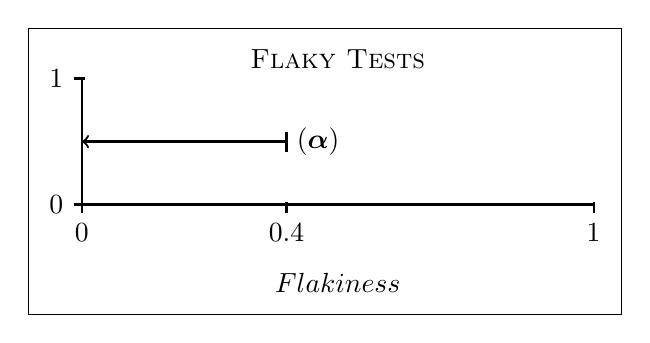
\begin{tikzpicture}[thick, framed, x=6.5cm, y=1.6cm]
	% Title
	\draw (0.5, 1) node[above] {$\textsc{Flaky Tests}$};

	% Axis
	\draw (0,0) -- coordinate (x axis mid) (1,0);
    \draw (0,0) -- coordinate (y axis mid) (0,1);

    % Axis Labels
    \node (padding) [below] at (0.4, 0) {};
	\node[below of = padding] at (x axis mid) {$Flakiness$};

    % Ticks
    \foreach \x in {0, 0.4, 1}
    	\draw (\x, 1pt) -- (\x, -3pt) node[anchor=north] {\x};
    \foreach \y in {0, 1}
    	\draw (1pt, \y) -- (-3pt, \y) node[anchor=east] {\y};

	% Flaky test range
    \draw[<-] (0, 0.5) -- (0.4, 0.5); % Draw horizontal line
    \draw (0.4, 0.42) -- (0.4, 0.58); % Draw right vertical tab

    % Alpha label
    \node [right] at (0.4, 0.5) {$(\boldsymbol{\alpha})$};
\end{tikzpicture}


Test suite $f$ with flaky tests $f!$.
Budget $B_{f} = B_{6} + B_{f!} + B_{nd}$

\paragraph{Instrumentation pseudocode:}

% Use 'in' for-loop range notation rather than 'to'.
\renewcommand{\algorithmicto}{\textbf{in}}

% The {algorithm} wrapper is pretty unattractive as far as I'm concerned.
% Need to look into alternative ways of formatting this.
\begin{algorithm}
\caption{Allocate instrumentation budget across a test suite}
\label{alg1}
\begin{algorithmic}
	% Perhaps this should just take a single tests[]. We can query the element to determine its 'priority' (relative flakiness).
	% Or, could take a vector<test, flakiness> to be explicit.
	\STATE{\textbf{splatter} (budget, flakyTests[], allTests[])}
	\STATE{}
	\COMMENT{Need a function that looks at all the tests and their associated priorities, orders them and attaches an allowedBudget value in terms of the whole budget}
 	\WHILE{$budget \geq 0$}
 		% Simpler if the 'instrumentTest' function returns a value representing the amount of budget it actually used, rather than its remainder.
 		\STATE{$budget \gets budget - allowedBudget + \textbf{instrumentTest} (test, allowedBudget)$}
	\ENDWHILE
\end{algorithmic}
\end{algorithm}

\begin{algorithm}
\caption{Instrument a test with respect to a given budget}
\label{alg2}
\begin{algorithmic}
	\STATE{\textbf{instrumentTest} (test, budget)}
	% Should 'sites' just be a parameter?
	\STATE{$sites \gets test.instrumentationSites$}
	\FOR{$site$ \TO $sites$}
		% Should probably define a cost function (e.g. cost(instrumentationPoint)) and use that, rather than using an unexplained accessor.
		\STATE{$cost \gets site.cost$}
		\IF{$cost \le budget$}
			\STATE{$site.active \gets true$}
			\STATE{$budget \gets budget - cost$}
		\ELSE
			% Need to work out how to define new algorithmic-style macros (e.g. \BREAK)
			\STATE{\textbf{break}}
		\ENDIF
	\ENDFOR
	\RETURN{budget}
\end{algorithmic}
\end{algorithm}

% Focus on the interesting design decisions. For example, what were the alternatives, why select one particular solution?
% Don't flood the chapter with diagrams. Be selective.
% Avoid lengthy sections of code; use pseudo-code.
% This is a core chapter and will usually be quite substantial, 10 pages or more.
\section{Design and Implementation}
\label{sec:imp}

\begin{framed}
	\begin{itemize}
		\item Describe the design of what you have created.
		\item Start with the application architecture, giving its overall structure and the components that make up that structure.
		\item Give a description of the design of each of the components that make up the architecture.
		\item Include the database or storage representation.
		\item Provide implementation details as necessary.
	\end{itemize}
\end{framed}

% This chapter will typically be 2-4 pages in length but could be more depending on the depth of testing done.
\section{Testing}
\label{sec:testing}

\begin{itemize}
	\item Describe your testing strategy (unit, functional, acceptance testing and how they are carried out). How were test cases selected?
	\item Examples of specific tests and how they were carried out (e.g., using mock objects to break dependencies). Focus on the interesting cases.
	\item A summary of the test results and what coverage was achieved. The detailed test report(s) should appear in the appendix.
	\item If your project requires substantial evaluation of data and results, or other forms of testing that are not code-based, then adapt this chapter to suit.
\end{itemize}

\section{Evaluation}
\label{sec:eval}

\subsection{The problem is real: it occurs in real world test suites. The goal is to quantify the problem for the skeptical reviewer.}

\subsection{How serious/extensive is the problem?}

\subsection{We solve the problem}

\section{Related Work}
\label{sec:relwork}

Liblit’s Adaptive Bug Isolation [] and other papers have taken a conservative
approach to information gathering. The projects have targeted production code,
so privacy and performance are major concerns.

\todo{Citations - there are a lot to add here!}

\subsubsection{Ordering}

In previous statistical bug isolation projects, ordering is completely discarded
due to privacy concerns []. Recording a play-by-play execution is invasive to
the common user.

Since our instrumentation will run in a development environment, there are no
user concerns - the tests are automated. We can maintain ordering with a little
more overhead.

Multi-threaded environments are commonplace. In order to record the execution
order of multiple threads, we include the system time in each log event. Each
thread logs to a separate sink. After the tests run completes, we merge and
interleave the individual logs before storing them. We end up with a single log
file with times and thread IDs.

\subsubsection{Storage/Result Collection}

Again, the context of our execution allows more flexibility. In production
systems, logs have to be stored on user devices and (eventually) transferred to
a central location for analysis. User storage space and bandwidth is precious,
so it is essential to minimise both.

In our case, tests will be run internally on project-owned machines and devices.
Log files can be transferred to the central database immediately following a
test run. Each test run by definition requires a clean device, so build agents
will almost certainly never run out of space since they will at any moment be
storing the logs from at most one test run.

The only real storage concern is that of the central database. But, this can be
managed effectively by limiting the number of historical test run logs to keep -
much in the same way Jenkins and other CI tools do by default.

\subsubsection{Performance}

Instrumentation adds performance overhead. In the case of a production system,
this is a major problem since performance directly affects a user’s experience.
Nainar and Liblit \cite{ArumugaNainar:2010:ABI:1806799.1806839} propose an
adaptive bug isolation system with a performance overhead of just 1\%.

In a test environment, smoothness and load times rarely matter. Of course, there
are exceptions (performance regression tests, etc.), but we expect to mainly be
dealing with system tests. We can safely add instrumentation and ignore
performance, unless it begins to affect the thread-wise execution. If a \flaky
test begins consistently passing when heavily instrumented, we can simply reduce
the instrumentation until the previous \flaky behaviour is once again observed.

\subsubsection{Adaptivity}

Both fixed and adaptive approaches have been proposed[] in the past. All of
these approaches were developed with the underlying constraint of deploying the
instrumented software to real users. [adaptive bug isolation] makes use of
binary instrumentation to iteratively re-instrument deployed applications to
hone in on a bug-predicting predicates. Whilst the adaptive approach has many
benefits in terms of overhead, it relies on a specialized API - Dyninst - for
code patching to support the injection of  instrumentation at runtime. This has
additional runtime costs \cite{DyninstGuide} associated with saving and
restoring registers and performing protective checks not present in a fixed
instrumentation.

Again, our context allows more freedom. Every run requires a new build by
nature, so simply apply a unique fixed instrumentation every time. In other
words, we retain the optimisation benefits of a fixed instrumentation whilst
gaining those of the adaptive solution.

% This chapter is typically 204 pages long but could be longer if the project work requires more extensive evaluation.
\section{Conclusion}
\label{sec:conc}

\begin{itemize}
	\item A summary of what the project has achieved. Address each goal set out in the introduction.
	\item A critical evaluation of the results of the project (e.g., how well were the goals met, is the application fit for purpose, has good design and implementation practice been followed, was the right implementation technology chosen and so on).
	\item Future work. How could the project be developed if you had another 6 months.
	\item Wrap-up and final thoughts on your project.
\end{itemize}
\section{Appendix}
\label{sec:appendix}

\subsection{\venera System Manual}

Venera is a command-line tool that hooks into any Android test runner and
instruments your application test suite. It adds event-firing probes at instance
method entries and logs to a human-readable JSON format. Included is an SDK with
an annotation that gives developers control over the instrumentation policy.
Complex probes have a large overhead, but record a huge amount of program state.
Simple probes simply fire events. In the future, probes placement will be based
on historical test run data and a budget.

\subsubsection{Requirements}

To build the project from source, the following tools are required:

\begin{itemize}
  \item Java Development Kit (v.7+) \cite{jdk}
  \item Android SDK (with the latest tools) \cite{androidSDK}
  \item Gradle (v.1.10+) \cite{gradle}
\end{itemize}

We recommend using IntelliJ \cite{intellij}, Android Studio \cite{androidStudio}
or some other Java-centric IDE, although anything is fine in principal.

\subsubsection{Running the Project}

To try \venera on the included Android application (skeleton-android-app), run
from the command line:

\begin{lstlisting}[numbers=none]
cd skeleton-android-app
gradle clean connectedAndroidTest -P=venera
\end{lstlisting}

IntelliJ users can create a skeleton-android-app Gradle build configuration and
run the task {\tt clean connectedAndroidTest} with script parameters {\tt
-P=venera}.

To run \venera on your own Android application, modify the {\tt build.gradle}
file under the {\tt venera-instrumentation} directory to point to your APKs.
You'll need to also provide a Gradle task (or equivalent) to pull the results
from the device in the same way that skeleton-android-app's build.gradle already
does. Note that integration with other Android applications will be made more
intuitive in the future.


\subsection{\jenkinsPlugin System Manual}

The \jenkinsPlugin maintains a HSQL database of standard test artifacts
and their associated Venera JSON logs. It will eventually be responsible for
\venera result presentation and analysis.

\subsubsection{Source Code}

The full source code is freely available at \cite{heisentestPlugin}.

\subsubsection{Requirements}

To build the project from source, the following tools are required:

\begin{itemize}
  \item Java Development Kit (v.7+) \cite{jdk}
  \item Maven (v.3+) \cite{maven}
\end{itemize}

We recommend using IntelliJ \cite{intellij} or some other Java-centric IDE,
although any editor is fine in theory.

\subsubsection{Running the Project}

From the command line:

\begin{lstlisting}[numbers=none]
mvn hpi:run
\end{lstlisting}

IntelliJ users can create a build configuration with type Maven and working
directory set to the root of the project to execute the same command.

\subsubsection{Common Problems}

When executing mvn hpi:run I get {\lq}java.net.BindException: Address already in
use{\rq}.

Something is using the TCP port (probably a previous instance that failed to
shut down correctly). On Linux, running {\tt lsof -i tcp:\$PORT} will give you
the list of processes using TCP port {\tt\$PORT}, which you can then kill with
{\tt kill \$PID}.


\subsection{Supporting Data}

\subsubsection{Full Dalvik Bytecode Example}
\label{sec:sec:full_dalvik_bytecode_example}

\begin{lstlisting}
#1              : (in Lcom/example/MainActivity;)
  name          : 'anExampleMethod'
  type          : '(Ljava/lang/String;I)Ljava/lang/String;'
  access        : 0x0002 (PRIVATE)
  code          -
  registers     : 4
  ins           : 3
  outs          : 2
  insns size    : 5 16-bit code units
024570:                  |[024570] com.example.MainActivity.anExampleMethod:(Ljava/lang/String;I)Ljava/lang/String;
024580: 7120 8503 3200   |0000: invoke-static {v2, v3}, Lcom/example/MainActivity;.appendIntToString:(Ljava/lang/String;I)Ljava/lang/String; // method@0385
024586: 0c00             |0003: move-result-object v0
024588: 1100             |0004: return-object v0
      catches   : (none)
      positions :
        0x0000 line=22
      locals    :
        0x0000 - 0x0005 reg=1 this Lcom/example/MainActivity;
        0x0000 - 0x0005 reg=2 firstArg Ljava/lang/String;
        0x0000 - 0x0005 reg=3 secondArg I
\end{lstlisting}

\subsection{Project Plan and Interim Report}

\newcounter{oldSectionCounter2}
\newcounter{oldPageCounter2}

\setcounter{oldSectionCounter2}{\value{section}}
\setcounter{oldPageCounter2}{\value{page}}

% Set the current value of section to 0
\setcounter{section}{0}

\title{
	Improving Diagnostic Data Gathering for Problematic System Tests:\\
	\itshape{Project Plan}
}
\author{
	Morrison Cole\\
	\texttt{zcabg19@ucl.ac.uk}
	\and
	Supervisor: Dr Earl Barr\\
	\texttt{e.barr@ucl.ac.uk}
	\and
	External Supervisor: Colin Vipurs\\
	\texttt{colin.vipurs@shazam.com}
}
\date{November 13, 2013}

\maketitle

\section{Aims}

\begin{enumerate}
	\item{
		To detect any flaky\footnote{A \flaky test is one that fails intermittently for no obvious reason.} tests present in a test suite, by storing and analysing the results of historical builds on a continuous integration server, so that they may be brought to the attention of developers at Shazam to encourage the upkeep of a stable build.
	}
	\item{
		To automatically, for some non-trivial subset of the \flaky tests in a test suite, extract information that speeds their resolution, either by fixing the test case(s) or the tested program, for a reasonable cost.
	}
\end{enumerate}

\section{Objectives}

\begin{enumerate}
	\item{
		Manually study the \flaky tests present at Shazam. Understand how these tests fit into the bigger picture --- consider developer workflow, number of tests, type of tests, code coverage, and ratio of black to white box testing. Find out if developers consider these tests to be a problem themselves.
	}
	\item{
		Develop software to:
		\begin{enumerate}
			\item{
				Pre-process JUnit-style test results from a build, so that they may be persisted in a database for analysis.
			}
			\item{
				Determine, over a set test runs, which tests are \flaky. Attempt to detect trends --- common failure causes, etc. --- using statistical tools such as R and Weka.
			}
			\item{
				Produce a customisable visual representation of the detected \flaky tests for each build. Attach any relevant diagnostic information to each data point.
			}
		\end{enumerate}
	}
	\item{
		Review published research in the problem space – namely, studies aiming to improve diagnostic information from runtime crashes/errors. Techniques and ideas developed in these projects will no doubt be useful to us.
	}
	\item{
		Develop instrumentation (using a tool such as Java MOP or ASM) to automatically gather information that will be useful for developers investigating a particular test with the aim of making it stable.
	}
\end{enumerate}

\section{Deliverables}

\begin{enumerate}
	\item{
		An overview of the state of the test suites across the teams at Shazam. As well as this specific case, the industry as a whole should be considered. The impact that \flaky tests have upon the productivity of software teams should be discussed.
	}
	\item{
		A tested, documented Jenkins\footnote{Jenkins is an open source continuous integration tool written in Java. It has a rich library of existing plugins and is used at Shazam, as well as at countless other commercial software companies.} plugin that fulfils objective 2, customized to display the data that Shazam wants to see. This will be deployed at Shazam as early in the project as possible. This will be submitted publicly to the Jenkins project in the hope that it is accepted to the official list of plugins.
	}
	\item{
		Literature survey describing current research in the space detailed in objective 3. Cover any non-trivial techniques or tools that we use that may be difficult for an unfamiliar reader to grasp.
	}
	\item{
		Develop a technique to instrument the \flaky tests whilst avoiding altering the runtime execution as much as possible. This could be done (for example) by selecting random samples of the complete instrumentation, running the tests in question multiple times, and reconstructing the complete instrumentation from the set of runs.
	}
\end{enumerate}

\section{Work Plan}

\begin{center}
    \begin{tabular}{ | l | p{6cm} |}
    \hline
    Period & Work \% \\ \hline
    Project start to end October (4 weeks) & Literature search and review. Define IP terms with Shazam. \\ \hline
    Mid-October to mid-November (4 weeks) & Literature review continued. Software and tools researched and familiarised. Access to Shazam's codebase gained. \\ \hline
    November (4 weeks) & Jenkins plugin started. Literature review continued. \\ \hline
    End-November to mid-January (8 weeks) & Jenkins plugin finished and deployed at Shazam. Work on \flaky test instrumentation started. Interim report written. \\ \hline
    Mid-January to mid-February (4 weeks) & Iterate on Jenkins plugin based on Shazam's feedback (if necessary). Continue work on \flaky test instrumentation. \\ \hline
    Mid-February to end of March (6 weeks) & Jenkins plugin submitted to the Jenkins project. \flaky test instrumentation complete. Final report. \\ \hline
    \end{tabular}
\end{center}

\newpage

% Restore the old value of the section counter
\setcounter{section}{\value{oldSectionCounter2}}
\setcounter{page}{\value{oldPageCounter2}}
\newcounter{oldSectionCounter}
\newcounter{oldPageCounter}

\setcounter{oldSectionCounter}{\value{section}}
\setcounter{oldPageCounter}{\value{page}}

% Set the current value of section to 0
\setcounter{section}{0}

\title{
	Improving Diagnostic Data Gathering for Problematic System Tests:\\
	\itshape{Interim Report}
}
\author{
	Morrison Cole\\
	\texttt{zcabg19@ucl.ac.uk}
	\and
	Supervisor: Dr Earl Barr\\
	\texttt{e.barr@ucl.ac.uk}
	\and
	External Supervisor: Colin Vipurs\\
	\texttt{colin.vipurs@shazam.com}
}
\date{January 22, 2014}

\maketitle

\section{Progress So Far}

\begin{enumerate}
	\item{
		Reviewed existing literature in the research space. In particular, the work of Ben Liblit (Bug Isolation via Remote Program Sampling, Statistical Debugging of Sampled Programs).
	}
	\item{
		Negotiated a satisfactory verbal agreement with Shazam which states rather broadly that:
		\begin{enumerate}
		\item{\itshape they understand that we are academics who wish to publish certain information};
		\item {\itshape we understand that Shazam will not allow information that may negatively impact the business to be released publicly}.
		\end{enumerate}
	}
	\item{
		Received VPN credentials to access Shazam's internal Continuous Integration and Version Control so that the project can be worked on campus.
	}
	\item{
		Wrote scripts to pull both new and historical build results from Shazam's Continuous Integration servers. Have been running these and storing the data so that we can analyze it later.
	}
	\item{
		Set up a project Git repository / Wiki and began development of a Jenkins plugin. All code has been test driven from the Unit Test level so far, and has been written with as little coupling to Jenkins as possible. The plugin currently runs as a post-build step, parses all JUnit-style results and persists them in a database.
	}
	\item{
		Have begun to look at open-source projects for other examples of flaky tests - Mozilla's Tinderbox Build Log in particular. Any particularly interesting cases have been noted on the project Wiki.
	}
\end{enumerate}

\newpage

\section{Future Plans}

\begin{enumerate}
	\item{
		Complete the remaining features of the Jenkins Plugin:
	}
	\begin{enumerate}
		\item{
			Using Weka / R, analyse the test suite historically and attempt to detect useful trends such as common failure causes.
		}
		\item{
			Produce an output Web page that displays the flaky tests and any relevant diagnostic information.
		}
	\end{enumerate}
	\item{
		Continue gathering data on flaky tests at Shazam and at least two other projects / organisations. This means collecting developer statements, finding examples of flaky tests in open-source projects, documenting developer workflow etc.
	}
	\item{
		Develop a system to instrument Java code such that we share the cost of automatically gathering additional runtime information over multiple test-runs and are able to aggregate it afterwards.
	}
\end{enumerate}

\newpage

% Restore the old value of the section counter
\setcounter{section}{\value{oldSectionCounter}}
\setcounter{page}{\value{oldPageCounter}}

\subsection{Partial Code Listing}

This section lists a significant portion of the source code that makes up
\venera. Reading code on paper is not ideal --- we suggest checkout out the full
\venera source code with {\tt git} from \cite{heisentestInstrumentation} and the
\jenkinsPlugin source code from \cite{heisentestPlugin}.

\begin{landscape}
\lstinputlisting{../venera/venera-instrumentation/src/./main/java/com/heisentest/venera/Main.java}
\lstinputlisting{../venera/venera-instrumentation/src/./main/java/com/heisentest/venera/VeneraApkProcessor.java}
\lstinputlisting{../venera/venera-instrumentation/src/./main/java/com/heisentest/venera/VeneraApkInstrumenter.java}
\lstinputlisting{../venera/venera-instrumentation/src/./main/java/com/heisentest/venera/transform/dex/VeneraDexTransformer.java}
\lstinputlisting{../venera/venera-instrumentation/src/./main/java/com/heisentest/venera/transform/dex/visitor/SimpleInstanceMethodEntryMethodVisitor.java}
\lstinputlisting{../venera/venera-instrumentation/src/./main/java/com/heisentest/venera/transform/dex/visitor/VeneraRegisterAllocatingMethodVisitor.java}
\end{landscape}


%% Citations

% Causes all items in the database to be included in the references, regardless of whether or not they are cited.
\nocite{*}

% TODO: Check with Earl what citation style we want.
\bibliographystyle{abbrvnat}
\bibliography{Bib/paper}

\end{document}
